\documentclass[conference]{IEEEtran}
\newcommand*{\rootPath}{../}
\usepackage{url}

% math and cs
% \usepackage[]{algorithm2e}
\usepackage[linesnumbered,lined,boxed,commentsnumbered]{algorithm2e}
\usepackage{amsmath}
\usepackage{amssymb}
\usepackage{mathrsfs}
\newtheorem{definition}{Definition}
\newtheorem{proposition}{Proposition}
\newenvironment{proof}[1][Proof]{\begin{trivlist}
  \item[\hskip \labelsep {\bfseries #1}]}{\end{trivlist}}
  % \newenvironment{definition}[1][Definition]{\begin{trivlist}
  % \item[\hskip \labelsep {\bfseries #1}]}{\end{trivlist}}
  % \newenvironment{example}[1][Example]{\begin{trivlist}
  % \item[\hskip \labelsep {\bfseries #1}]}{\end{trivlist}}
  % \newenvironment{remark}[1][Remark]{\begin{trivlist}
  % \item[\hskip \labelsep {\bfseries #1}]}{\end{trivlist}}

% style
\usepackage{booktabs}
\usepackage{multirow}
\usepackage{lipsum}
\usepackage{todonotes}
\usepackage{standalone}
\usepackage{import}
\usepackage{url}
%\Urlmuskip=0mu plus 1mu %bug url

% graph
\usepackage{graphicx}
\usepackage[outdir=./]{epstopdf}
\usepackage[labelformat=simple]{subcaption}
\usepackage{array}
%\usepackage[colorinlistoftodos]{todonotes}
\newcommand{\HRule}{\rule{\linewidth}{0.5mm}}



\DeclareCaptionLabelSeparator{periodspace}{.\quad}
\captionsetup{font=footnotesize,labelsep=periodspace,singlelinecheck=false}
\captionsetup[sub]{font=footnotesize,singlelinecheck=true}


\usepackage[english,american]{babel}



\usepackage[capitalise,nameinlink]{cleveref}
%Nice formats for \cref
\crefname{section}{Sect.}{Sect.}
\Crefname{section}{Section}{Sections}
\crefname{figure}{Fig.}{Fig.}
\Crefname{figure}{Figure}{Figures}

\usepackage{xspace}
%\newcommand{\eg}{e.\,g.\xspace}
%\newcommand{\ie}{i.\,e.\xspace}
\newcommand{\eg}{e.\,g.,\ }
\newcommand{\ie}{i.\,e.,\ }


\renewcommand\thesubfigure{(\alph{subfigure})}


%invert table
\usepackage{collcell}
\usepackage{datatool}
\usepackage{environ}


\standalonetrue

\begin{document}

%%=============================================================================




\section{Notre syst\`eme de vote}
\label{sec:laprimaire}

Le syst\'eme de vote utilis\'e sur laPrimaire.org part du syst\`eme de vote du JM. Ce syst\`eme n'est pas adapt\'e pour un grand nombre de candidats, puisque tous les \'electeurs ne peuvent pas passer autant de temps \'a juger chaque candidat par soucis de temps.

\subsection{Fonctionnement}
L'\'election se d\'eroule en deux phases. Lors de la premi\'ere phase, les \'electeurs devront juger seulement un lot de 10 candidats, plut\^ot que de s'exprimer sur chaque candidat. Le nombre de 10 candidats correspond \'a la moyenne du nombre de candidats aux \'elections pr\'esidentielles depuis la r\'eforme du vote en 1962.

A l'issue de ce scrutin, les cinq candidats les mieux class\'es seront qualifi\'es. Nous avons choisi le chiffre cinq pour repr\'esenter plus de tendances politiques que lors du second tour aux \'elections pr\'esidentielles. 

Nous avons ajout\'e un quorum \'a la qualification: pour chaque candidat qualifi\'e, la moiti\'e de ses jugements ne doit pas \^etre D\'efavorable. Ce quorum sert \`a disqualifier les candidats trop clivants. Le seuil de $50\%$ a \'et\'e plac\'e haut pour d\'ecourager des strat\'egies de disqualifications. Par exemple si le seuil \'etait \`a $5\%$, les soutiens d'un candidat pourraient plus facilement s'unir pour disqualifier un autre candidat.

Lors de la seconde phase, les \'electeurs pourront juger pour tous les candidats qualifi\'es \`a l'aide du jugement majoritaire.


\subsection{Proc\'edure pour construire les lots}

Pour ne pas truquer la phase de qualification, les lots de 10 candidats sont choisis \'a l'avance et les \'electeurs ne pourront pas choisir les candidats qu'ils jugeront lors du premier tour. Pour que cette phase ne soit pas truqu\'ee, trois conditions ont \'et\'e s\'electionn\'ees.

\begin{enumerate}
  \item \emph{Le nombre d'apparition de chaque candidat dans les lots est le m\^eme.} Pour le vote majoritaire, ne pas apparaitre le m\^eme nombre de fois cr\'e\'e un biais important : si un candidat A re\c{c}oit $100\%$ des votes, mais n'apparait que dans $10\%$ des lots, il perdera contre un candidat B qui ne re\c{c}oit que $20\%$ des votes, mais qui apparait dans $100\%$ des lots. Pour le jugement majoritaire, ne pas recevoir strictement le m\^eme nombre de jugements n'influe pas sur le classement g\'en\'eral gr\^ace \`a l'utilisation de la m\'edianne. En revanche, le nombre de jugements doit rester le plus proche possible pour garantir la repr\'esentativit\'e du vote. 
  \item \emph{Chaque candidat a la m\^eme probabilit\'e de rencontrer tout autre candidat dans un lot.} Un biais cognitif dans les jugements consiste \`a juger un candidat par rapport \`a un autre : lorsqu'un \'electeur juge un candidat, il se r\'ef\`ere aux jugements qu'il a exprim\'e pr\'ec\'edemment. Il est donc important de veiller \`a ce que chaque candidat rencontre n'importe quel autre candidat. 
  \item Le classement est le m\^eme que si tous les \'electeurs jugent attentivement et ind\'ependemment chaque candidat. 
\end{enumerate}

Ces conditions sont d'autant plus difficiles \`a respecter que le nombre d\'electeurs n'est pas connu \'a l'avance : les \'electeurs peuvent s'inscrire \`a l'\'election, mais finalement ne pas y participer. Ainsi, une construction au pr\'ealable des lots n'est pas possible: si une part significante des \'electeurs qui s'expriment sur un candidat ne sont pas pr\'esents lors de l'\'elections, alors ce candidat ne recevrait pas autant de jugements qu\'un autre.

C'est pourquoi, la construction des lots se fait pendant le vote. Nous avons test\'e la proc\'edure suivante qui donne de bons r\'esultats:
Pour chaque lot, la proc\'edure consiste \`a :
\begin{enumerate}
  \item compter le nombre d'occurences $\#occ_i$ pour chaque candidat $i$ dans les lots pr\'ec\'edents ;
  \item construire un tableau qui attribut \`a candidat $i$ la valeur $1/\#occ_i$ si $\#occ_i \ne 0$ et $1$ sinon ;
  \item normaliser ce tableau en le divisant par la somme de chacune de ses cases ;
  \item ce tableau forme la probabilit\'e qu'\`a un candidat d'\^etre choisi dans le prochain lot.
\end{enumerate}

\begin{figure*}[!ht]
  \centering
  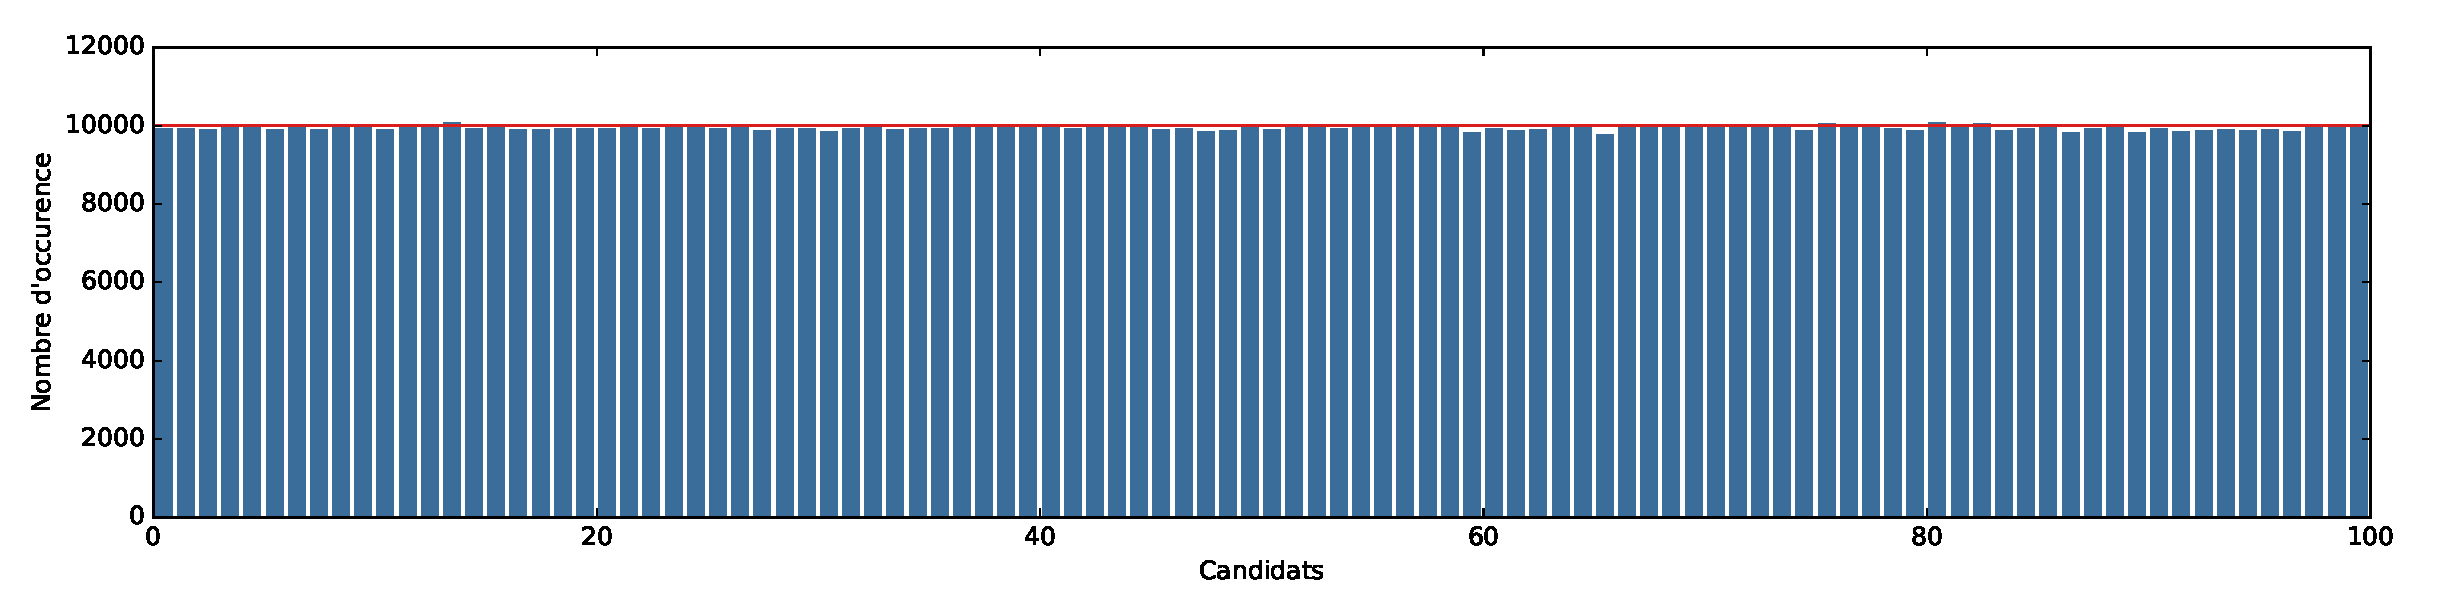
\includegraphics[width=0.98\textwidth]{../\rootPath image/lot_Nc-100_Ne-100000_Nl-10.pdf}
  \caption{Avec 100000 \'electeurs et 100 candidats, chaque candidat apparait autant de fois que les autres candidats dans les lots}
  \label{fig:candidatsVSoccurence}
\end{figure*}

Sur la \cref{fig:candidatsVSoccurence}, le nombre d'apparition de chaque candidat est repr\'esent\'e. Une ligne rouge repr\'esente la moyenne d'apparition. Chaque candidat n'apparait pas exactement le m\^eme nombre de fois, bien que l'\'ecart \`a la moyenne est visiblement faible. 

L'\'ecart-type, d\'efini comme la moyenne des \'ecarts \`a la moyenne d\'epend du nombre d\'electeurs : plus les \'electeurs sont nombreux, et plus l'\'ecart-type devient faible. L'\'ecart-type ne peut \^etre interpr\'et\'e que par rapport \`a la moyenne : un \'ecart-type de 1 et une moyenne de 10 signifient qu'en g\'en\'eral, le nombre d'apparition d'un candidat est de 10, bien qu'il peut souvent de 9 ou de 11. Le rapport \'ecart-type sur moyenne est en revanche plus facile \'a interpr\'eter car il correspond \`a un pourcentage de d\'eviation. Dans la \cref{fig:rem}, ce rapport est calcul\'e pour plusieurs tranches d\'electeurs. A partir de 30000 \'electeurs, ce rapport devient inf\'erieur \`a $1\%$. Autrement dit, l'\'ecart dans le nombre d'apparition de chaque candidat est n\'egligeable.


\begin{figure}[!ht]
  \centering
  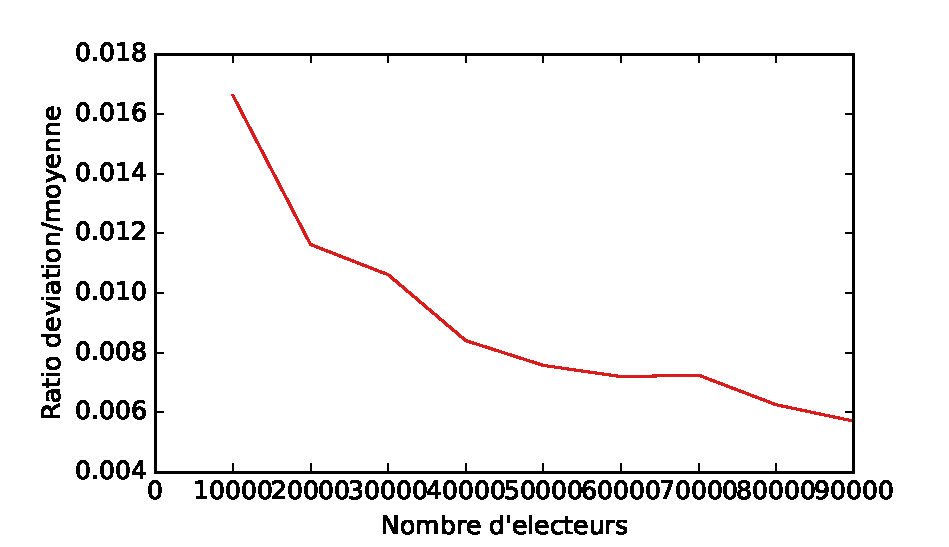
\includegraphics[width=0.98\columnwidth]{../\rootPath image/rsm_Nc-100_Nl-10.pdf}
  \caption{A partir de 30000 \'electeurs, le rapport \'ecart-type sur moyenne devient inf\'erieur \'a $1\%$.}
  \label{fig:rem}
\end{figure}

La premi\`ere condition est donc valid\'ee. La \cref{fig:corr} valide la seconde condition. Cette figure repr\'esente le nombre de fois qu'un candidat rencontre les autres candidats dans un m\^eme lot. La diagonale est quand un candidat se retrouve lui-m\^eme, ou plus simplement, quand il apparait dans un lot. Les valeurs sont donc les m\^emes que dans la \cref{fig:candidatsVSoccurence}. Le bleu quasi-uniforme montre qu'aucun biais est introduit dans la rencontre d'un candidat par rapport \`a un autre. Il reste \`a valider la derni\`ere condition.


\begin{figure}[!ht]
  \centering
  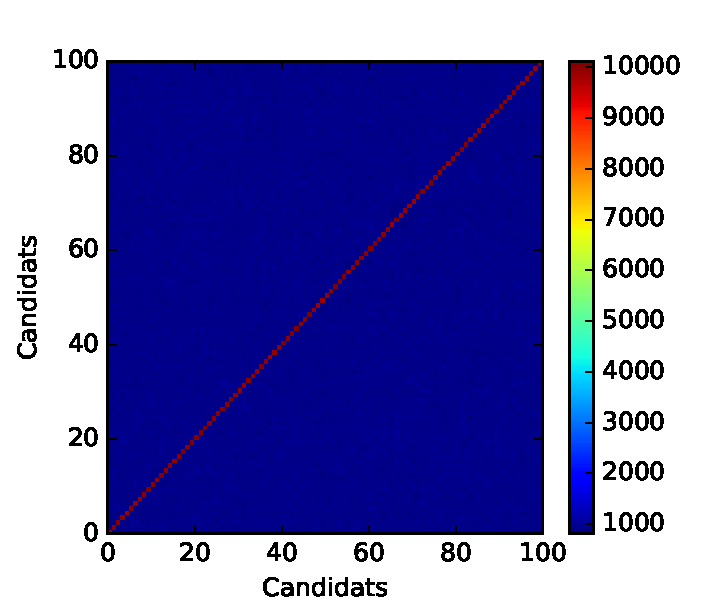
\includegraphics[width=0.98\columnwidth]{../\rootPath image/corr_Nc-100_Ne-100000_Nl-10.pdf}
  \caption{A partir de 30000 \'electeurs, le rapport \'ecart-type sur moyenne devient inf\'erieur \'a $1\%$.}
  \label{fig:rem}
\end{figure}

\subsection{Nombre minimum d'\'electeurs}

Le jugement majoritaire a \'et\'e con\c{c}u en supposant que les \'electeurs jugent tous les candidats. 

Pour montrer que ce syst\`eme fonctionne \'egalement lorsque les \'electeurs ne jugent qu'un lot de candidats, nous avons compar\'e le gagnant d'une premi\'ere phase o\`u tous les candidats sont jug\'es par tous les \'electeurs et une seconde phase o\`u les \'electeurs ne jugent que les candidats dans leur lot. Nous avons remarqu\'e qu'un nombre minimum d'\'electeurs selon le nombre de candidats est n\'ecessaire.

Le nombre minimum d'\'electeurs est estim\'e en calculant l'erreur moyenne de classement sur les 5 
\begin{figure}[!ht]
  \centering
  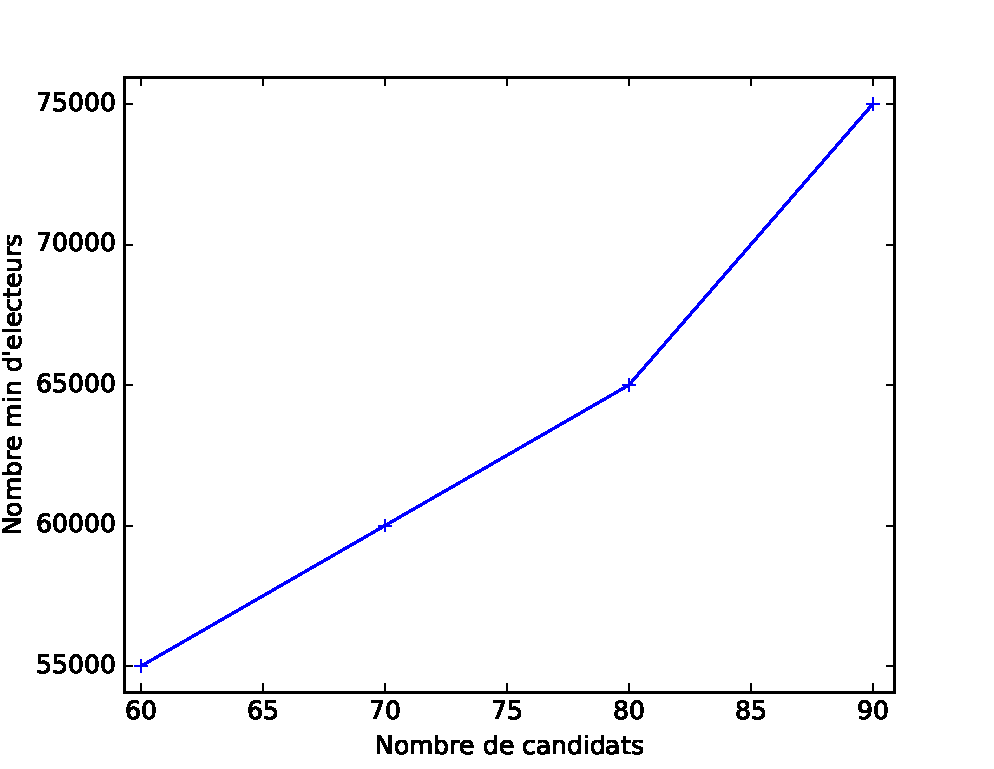
\includegraphics[width=0.98\columnwidth]{../\rootPath image/Nmin-electeurs.pdf}
  \caption{Le nombre minimal d'\'electeurs est donn\'e \`a 5000 \'electeurs pr\`es pour un nombre de candidats entre 60 et 90}
  \label{fig:rem}
\end{figure}

Dans la \cref{fig:rem}, l
\end{document}


